\documentclass [french, 12pt, a4paper, twoside] {report}
\usepackage[frenchb]{babel}
\usepackage[T1]{fontenc}
\usepackage[utf8]{inputenc}
\usepackage[hidelinks]{hyperref}
\usepackage{lettrine}
\usepackage{palatino}
\renewcommand*\rmdefault{ppl}
\usepackage{fancyhdr}
\usepackage{float}
\usepackage{wrapfig}
\usepackage{graphicx}
\usepackage{caption}
\usepackage{subcaption}
\usepackage{amsmath}
\usepackage{color}
\usepackage{url}
\usepackage{paralist}
\usepackage{titlesec}
\usepackage[sort, authoryear]{natbib}
\usepackage{listings}
\usepackage{placeins}

%% Bib
\bibpunct{[}{]}{,}{n}{,}{,}
\newcommand{\todo}[1]{\textbf{\color{red}TODO: #1}}
\newcommand{\benumline}{\begin{inparaenum}[\itshape i\upshape)]}
\newcommand{\eenumline}{\end{inparaenum}}
 %% Graphics
\graphicspath{{include/img/},{include/pdf/}}
\DeclareGraphicsExtensions{.jpeg,.jpg,.png}
%% Title
\titleformat{\chapter}[hang]{\bf\huge}{\thechapter}{2pc}{}
\titlespacing*{\chapter}{0pt}{0pt}{20pt}
%% subsubsection numbering
\setcounter{secnumdepth}{3}

%% Header / Footer
\fancyhead{}
\fancyfoot{}
\fancyhead[C]{\todo{title}}
\fancyhead[L,R]{{\color{red}Draft version}}
\fancyfoot[L]{Université Pierre \& Marie Curie}
\fancyfoot[C]{\thepage}
\fancyfoot[R] {Pierre-Yves PÉNEAU}
\renewcommand{\headrulewidth}{0.4pt}
\renewcommand{\footrulewidth}{0.4pt}

% correct bad hyphenation here
\hyphenation{}
\setlength{\topmargin}{0cm}
\setlength{\headheight}{1cm}
\setlength{\textheight}{23cm}
\setlength{\textwidth}{16cm}
\setlength{\oddsidemargin}{0cm}
\setlength{\evensidemargin}{0cm}
\setlength{\columnsep}{0.125in}
\setlength{\columnseprule}{0.5pt}
\setlength{\footskip}{1cm}

%% lst config
\definecolor{mygreen}{rgb}{0,0.6,0}
\definecolor{mygray}{rgb}{0.5,0.5,0.5}
\definecolor{mymauve}{rgb}{0.58,0,0.82}
\definecolor{lightgray}{gray}{0.9}
\lstset{ %
  backgroundcolor=\color{white},
  basicstyle=\footnotesize\ttfamily,     
  belowcaptionskip=1\baselineskip,
  breakatwhitespace=false,      
  breaklines=true,              
  captionpos=b,                 
  commentstyle=\color{mygreen}, 
  extendedchars=true,           
  frame=single, 
  keepspaces=true,
  keywordstyle=\color{blue},    
  language=C,                   
  %numbers=none,                 
  numbersep=5pt,                
  numberstyle=\tiny\color{mygray},
  rulecolor=\color{black},        
  showspaces=false,               
  showstringspaces=false,         
  showtabs=false,                 
  stepnumber=2,                   
  stringstyle=\color{mymauve},    
  tabsize=4,
  title=\lstname
  xleftmargin=\parindent,
}


%% \lstdefinestyle{almos}{
%%   backgroundcolor=\color{lightgray},
%%   keywordstyle=\bfseries\color{mygreen},
%%   commentstyle=\itshape\color{mymauve},
%%   identifierstyle=\color{black},
%%   %% stringstyle=\color{orange},
%%   morekeywords={pid_t, uid_t, gid_t,
%%     uint_t, uint16_t, uint32_t, uint64_t, spinlock_t, mcs_lock_t, atomic_t,
%%     bool_t, error_t, task_s, thread_s, cluster_s, cpu_s, list_entry, page_s,
%%     sig_mgr_s, event_s, rwlock_s, vmm_s, pmm_s, vfs_node_s, vfs_file_s,
%%     fd_info_s, metafs_s, wait_queue_s, mapper_s, vfs_stat_s, vfs_context_s,
%%     vfs_node_s, vfs_file_s, vfs_node_op_s}, }

\sloppy
%%%%%%%%%%%%%%%%%%%%%%%%%%%%%%%%%%%%%%%%%%%%%%%%%%%%%%%%%%%%%%%%%%%%%%%%
\def \printed {no}
\def \yes {yes}
\def \no {no}

\begin{document}

  \begin{titlepage}  

  {\begin{center}\huge\textsf{Université Pierre et Marie Curie}\end{center}}


  \vspace{0.4cm}
  

  {\begin{center}\huge\textsf{Mastère de sciences et technologies}\end{center}}
  
  \vspace{0.4cm}
  
  {\begin{center}\huge\textsc{Mention Informatique \\2014 -- 2015} \end{center}}
  
  \vspace{0.4cm}
  
  {\begin{center}\huge\textsf{Spécialité : SAR}\end{center}}
  
  {\begin{center}\large\textsc{Systèmes et Applications Répartis }\end{center}}
  
  \vspace{0.4cm}

  {\begin{center}\Huge\textbf{Ajout du mécanisme de migration de thread pour le
        multi-noyau ALMOS}\end{center}}
  
  \vspace{0.4cm}
  
  {\begin{center}\huge\textsc{Rapport de Pré-soutenance}\end{center}}
  
  \vspace{0.4cm}
  
  {\begin{center}\large\textsf {11 Mai 2015 }\end{center}}
  
  \vspace{0.4cm}
  
  {\begin{center}\Large\textsc{Présenté Par}\end{center}}
  
  {\begin{center}\huge\textsc{Pierre-Yves PÉNEAU}\end{center}}
  
  \vspace{0.4cm}
  
  {\begin{center}\Large\textsc{Encadrants}\end{center}}
  
  {\begin{center}\huge\textsc{Franck Wajsbürt}\end{center}}
  
  {\begin{center}\huge\textsc{Mohamed KARAOUI}\end{center}}
  
  {\begin{center}\large\textsf{Laboratoire d'accueil : LIP6 }\end{center}}
  
  {\begin{center}\large\textsf{Equipe ALSOC}\end{center}}
  
\end{titlepage}

  \pagestyle{headings}
  \setcounter{page}{1}
  \pagenumbering{Roman}


  %% For printed version
  \ifx \printed \yes
    \newpage
    \thispagestyle{empty}
    \mbox{}
  \fi

  \tableofcontents

  %% For printed version
  \ifx \printed \yes
  \newpage
  \thispagestyle{empty}
  \mbox{}
  \fi

  \listoffigures

  %% For printed version
  \ifx \printed \yes
  \newpage
  \thispagestyle{empty}
  \mbox{}
  \fi

  \clearpage
  \setcounter{page}{1}
  \pagenumbering{arabic}
  \pagestyle{fancy}
  \fancypagestyle{plain}{}

  \chapter{Introduction}

  \hspace{1cm}Au milieu des années 2000, les fabricants de processeurs ont
  atteint une limite technique.  Au-delà de 100 Watts par boitier, il est
  difficile de refroidir les circuits à l'aide de simples ventilateurs. Les
  technologies comme le water cooling~\citep{googleXXXXdatacenters} sont
  coûteuses et énergivores.  Pour continuer l'augmentation de puissance des
  processeurs en profitant de la loi de Moore, ils ont dû cesser de complexifier
  l'architecture des c\oe urs et d'augmenter leur fréquence de
  fonctionnement. Au contraire, ils ont simplifié les c\oe urs pour en mettre
  plusieurs par processeur.  De nos jours, les architectures à 8 c\oe urs sont
  courantes, celles à une cinquantaine de c\oe urs sont disponibles, et d'autres
  comportant plusieurs centaines, voire milliers, sont à prévoir.
  L'augmentation du nombre de c\oe urs par processeur permet l'augmentation du
  nombre d'instructions exécutées par cycle.  Cela impose une augmentation de la
  quantité de mémoire nécessaire et du débit des accès~\citep{hp2012z820,
    puget2013z9pe}. Les systèmes d'exploitation doivent s'adapter pour gérer
  efficacement ces nouvelles ressources.\\

  \hspace{1cm}Dans ce stage, l'architecture matérielle considérée est
  l'architecture TSAR~\citep{greiner2009tsar} développée au LIP6. TSAR est une
  architecture NUMA (\textit{Non Uniform Memory Acces}) à mémoire partagée
  cohérente, composée de 1024 c\oe urs 32 bits et 1To de mémoire physique (40
  bits).  Les c\oe urs sont répartis en clusters contenant chacun 4 c\oe urs et
  gérant un segment de 4Go de mémoire physique. Le choix de c\oe urs 32 bits, et
  non 64bits, est assumé. C'est, selon les architectes, le meilleur compromis en
  énergie dissipée par instruction et cela permet un meilleur usage des caches
  car les pointeurs sont plus petits.  Un système d'exploitation nommé
  ALMOS~\citep{almaless2011almos} a été spécialement développé pour TSAR. Ce
  système est basé sur un noyau monolithique, tout comme Linux ou *BSD. ALMOS
  signifie \textit{Advanced Locality Management Operating System}. En effet, son
  but premier est le placement efficace des données dans les segments mémoires,
  et des threads accédant à ces données sur les c\oe urs.\\

  \hspace{1cm}L'architecture TSAR utilisée lors du développement d'ALMOS n'était
  pas finalisée. Elle ne proposait que 4Go de mémoire physique (32 bits). Elle
  gère désormais 1To (40 bits). Le but de ce stage est de faire évoluer ALMOS
  pour permettre la gestion de ce tera octet.\\

  \hspace{1cm}Nous faisons face à plusieurs problèmes. Le premier est que les
  c\oe urs 32 bits sont limités à 4Go d'espace adressable virtuel. Le noyau doit
  gérer un espace mémoire physique supérieur à l'espace virtuel des
  processeurs. Pour résoudre ce problème, nous verrons que nous allons devoir
  répartir et souvent répliquer toutes les structures du noyau dans chaque
  cluster. \todo{ALMOS, dans sa version 32 bits, a déjà une organisation
    clusterisée pour gérer le co-placement des threads et des données, mais cela
    n'interdit pas d'accéder facilement à toute la mémoire, c'est désormais
    difficile.} Le deuxième problème est donc de revoir la répartition ou
  réplication des structures du noyau et leur mode d'accès. ALMOS va ainsi
  évoluer vers une structure semblable par certains aspects au
  multi-noyau~\citep{baumann2009multikernel}. Ainsi, le troisième problème est
  une conséquence du deuxième. Si certaines structures sont répliquées, il faut
  que le système en garantisse la cohérence et ainsi offre à l'utilisateur
  l'illusion d'un noyau monolithique. \\

  \hspace{1cm}Pour ce stage, nous allons nous concentrer sur les structures
  partagées par les threads d'un processus, telles que les descripteurs de
  fichiers ou les zones mémoires partagées. \\


  \hspace{1cm}Ce document est organisé de la manière suivante: dans le
  chapitre~\ref{chap:subject}, nous présenterons le sujet du stage et la
  problématique. Le chapitre~\ref{chap:sol} expliquera la solution envisagée
  pour ce répondre à la problématique. Ensuite, nous donnerons dans le
  chapitre~\ref{chap:tasks} le découpage des tâches identifié. Enfin, nous
  donnerons dans le chapitre~\ref{chap:tests} la procédure de recette qui sera
  utilisée pour valider notre solution, et dans le chapitre~\ref{chap:sched}
  l'échéancier retenu pour ce travail.

  \chapter{Sujet du stage}
\label{chap:subject}

  \section{Contexte de l'étude}

    Pour répondre à ces enjeux de passage à l'échelle et de consommation
    énergétique, l'équipe ALSOC du LIP6 participe à deux projets européens
    successifs: TSAR~\cite{tsar2008} et SHARP~\cite{sharp2012}. Ces projets,
    pour le LIP6, ont pour but de fournir une architecture de processeur, TSAR,
    de plusieurs centaines de c\oe urs, et un système d'exploitation pour gérer
    efficacement cette nouvelle architecture.

    Notre travail portera sur ALMOS, dont l'architecture va évoluer vers celle
    d'un multi-noyau, et plus particulièrement sur la migration de tâches entre
    différentes instances du noyau. Nous allons dans un premier temps présenter
    l'architecture matérielle TSAR. L'étude de cette dernière est essentielle
    pour bien comprendre les enjeux pour ALMOS. Ensuite nous présenterons le
    noyau ALMOS, et notamment son cycle de vie, et enfin nous concluerons sur le
    travail que nous allons effectuer dans le cadre de ce stage.
  

    \subsection{L'architecture TSAR}
    \label{sec:tsar}

      TSAR est l'architecture d’un processeur multi-c\oe urs cc-NUMA homogène
      pouvant intégrer jusqu’à 1024 c\oe urs~\cite{greiner2009tsar}. Cette
      architecture est le résultat de deux projets de recherche européens
      MEDEA+~\cite{tsar2008,sharp2012} dont les principaux partenaires
      industriels sont BULL, Philips et THALES, et dont les partenaires
      académiques sont le LIP6 et le CEA-Leti. La figure \ref{fig:tsar} est un
      aperçu global de l'architecture TSAR. Il s'agit d'un ensemble de clusters
      interconnectés par un NoC DSPIN. Chaque c\oe ur dispose de ses propres
      caches L1 indexés en adresses physiques (données et instructions
      séparéess) et d'une MMU. La cohérence des caches de premier niveau de tous
      les c\oe urs ainsi que des TLBs est assurée par un protocole matériel
      nommé DHCCP. Une description complète de cette architecture est disponible
      sur le site du projet TSAR~\cite{tsar2008web}.

      \begin{figure}[ht]
        \centering 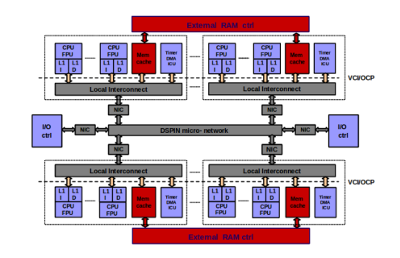
\includegraphics[scale=0.2]{include/img/tsar.png}
        \caption{Schéma global de l'architecture TSAR~\citep{greiner2009tsar}.}
        \label{fig:tsar}
      \end{figure}

      Dans la suite de ce document, on considére la version TSAR-Leti comme
      étant l'architecture de référence. Celle-ci contient jusqu'à 1024 c\oe urs
      MIPS32 répartis en 256 clusters de 4 c\oe urs chacun. La mémoire physique
      adressable est de 1To, et chaque cluster gère un segment de 4Go


    \subsection{Le noyau ALMOS}
    \label{sec:almos}

      Le noyau ALMOS~\cite{almaless2011almos,almaless2014universite} est un
      noyau monolithique expérimental developpé au LIP6 par l'équipe ALSOC
      depuis 2011. Sujet de thèse de Ghassan Almaless, le développement est
      maintenant à la charge de Mohamed Karaoui (système de fichiers) et Clément
      Devigne (exécution de machines virtuelles). Le but d'ALMOS est de répondre
      à la problématique de la localité des accès mémoires dans les machines
      cc-NUMA. Une des particularités dans les choix architecturaux d'ALMOS est
      d'avoir développé un noyau monolithique. Il respecte la norme
      POSIX~\cite{posix2013} et implémente différentes libraires:
      \texttt{libpthread, mpi, openMP}\ldots Le but premier d'ALMOS est de
      garantir un passage à l'échelle et une conservation de la localité des
      accès mémoires. Pour cela, le noyau intègre trois nouveaux mécanismes:
      \benumline \item les clusters managers \item les réplica-noyau \item une
      nouvelle stratégie d'allocation mémoire (\textit{Auto-Next-Touch})
      \eenumline.


    \subsection{Limitations de la version initiale}

      Développé initialement sur une architecture avec 4Go de mémoire physique,
      le noyau ne peut pas supporter plus de 4Go de mémoire vive. L'objectif
      visé n'était pas de supporter le tera-octet de mémoire de TSAR, mais de
      supporter le passage à l'échelle de plusieurs centaines de c\oe
      urs. Ainsi, un des premiers problèmes d'ALMOS est le mapping de l'espace
      virtuel. En effet, lors de la phase de boot, ce dernier cherche à mapper
      toute la mémoire physique du cluster de boot dans son espace
      virtuel. Contraitement aux noyaux ``classiques'', ALMOS s'accorde 2Go
      d'espace virtuel au lieu de 1. Donc, si ce cluster possède (au moins) 2Go
      de mémoire physique, l'ensemble du noyau est mappé dans ce seul
      cluster. Enfin, cela ne laisse que 2Go de mémoire virtuelle pour les
      applications utilisateur.


    \subsection{Contributions de François \citeauthor{guerret2014exploitation}}

      La gestion d'une telle quantité de mémoire fût le sujet de stage de
      François~\citet{guerret2014exploitation} en 2014. Ce dernier proposa
      différents changements pour ALMOS (figure~\ref{fig:almos-guerret}) :
      \benumline \item réduire l'espace virtuel noyau à 1Go \item répartir cet
      espace virtuel entre les clusters \item sortir de l'espace virtuel les
      structures de données du noyau de taille importante \eenumline.

      \begin{paragraph}{Répartition de l'espace d'adressage noyau:}
        Elle est calculée en fonction du nombre de clusters de l'architecture
        ($\frac{\text{Taille virtuelle}}{\text{Nb clusters}}$). Pour une
        architecture TSAR-Leti 40 bits, on dispose de 256 clusters, on a donc
        $\frac{1000}{256}\approx4$Mo d'espace virtuel pour le noyau par cluster.
      \end{paragraph}

      \begin{figure}[ht]
        \centering 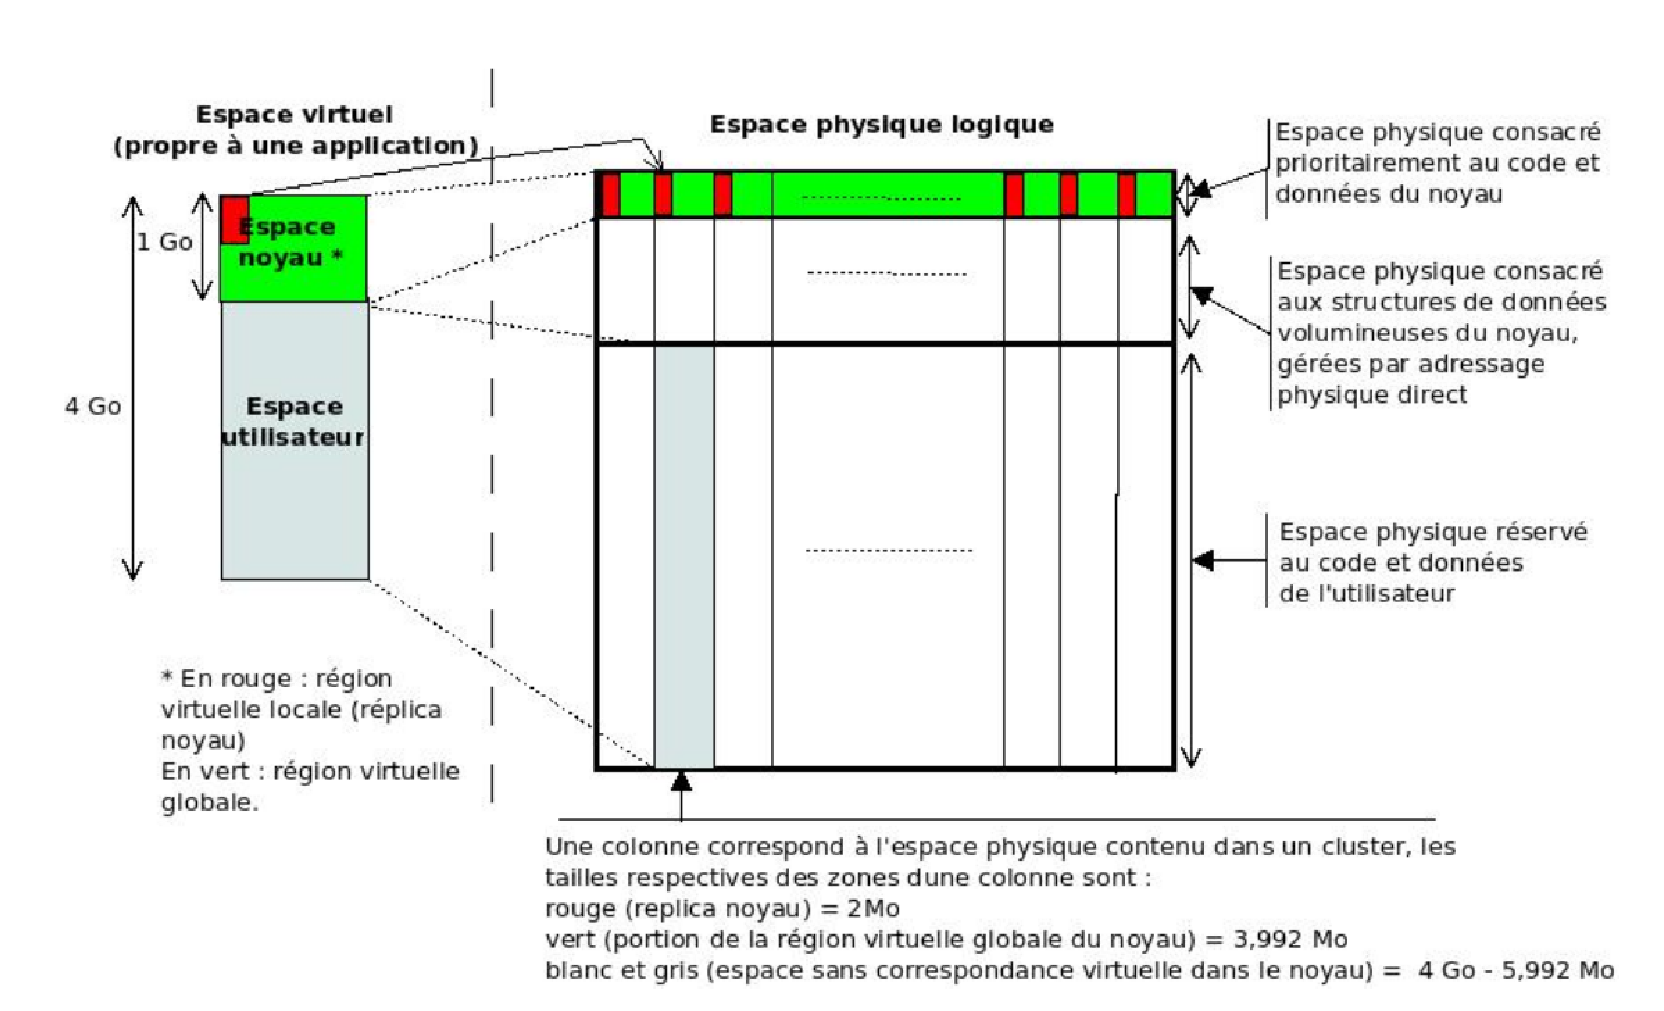
\includegraphics[scale=0.3]{include/img/almos-guerret}
        \caption{Répartition de l'espace virtuel du noyau tel que proposé par
          François \citet{guerret2014exploitation}.}
        \label{fig:almos-guerret}
      \end{figure}

      \begin{paragraph}{Gestion en adressage physiques de structures de données:}
        Avec seulement 4Mo d'espace virtuel pour le noyau par clusters,
        certaines structures de données ne pouvent plus être contenues dans un
        si petit espace, comme par exemple la table des pages d'un
        processus. Celle-ci, une fois pleine\footnote{Ce cas n'arrive jamais,
          mais il est néanmoins théoriquement possible}, peut atteindre une
        taille maximale de 8Mo. De plus, chaque processus dispose de sa propre
        table des pages. Il est techniquement impossible de stocker 8Mo dans
        4Mo, François a donc choisi de sortir cette structure de l'espace
        virtuel.

        La seconde structure de données problématique est la table des
        descripteurs de pages physiques. Les noyaux monolithiques, dont ALMOS,
        ont fait le choix de décrire dans une structure à plat toutes les pages
        physiques qu'offre la mémoire. Ainsi, pour décrire le tera-octet de
        mémoire offert par TSAR, il est nécessaire d'utiliser 14Go de mémoire,
        soit 56Mo par cluster. Une fois de plus, il est impossible de stocker
        cette structure dans l'espace virtuel noyau. Celle-ci en a donc été
        sortie, et est gérée en adressage physique.
      \end{paragraph}

      \begin{paragraph}{Résultats:}
        Ce travail n'a malheureusement pas donné lieu à une solution
        fonctionnelle. La gestion par des adresses physiques de ces deux
        structures s'est avérée être très compliquée et nécessitait de recoder
        une partie conséquente du noyau. Le principal inconvénient de ce choix
        est le parcours de listes: il est nécessaire de vérifier que chaque
        élément n'est pas une structure gérée physiquement avant de pouvoir y
        accéder. Cela allourdi considérablement l'opération, cette solution fût
        donc abandonnée. Néanmoins, elle a posée les bases de la version
        suivante d'ALMOS.
      \end{paragraph}


  \section{Définition et analyse du problème}      

    \subsection{Passage au mode multi-noyau}
    \label{sec:multi-noyau}

      La version actuelle d'ALMOS proposée par Mohamed Karaoui supprime
      totalement l'espace virtuel pour le noyau. Ce dernier fonctionne
      entièrement en adressage physique et de ce fait passe en mode multi-noyau,
      avec une instance de noyau par cluster. Ces changements permettent de
      gérer toute la mémoire physique de la plateforme TSAR, puisque:
      \benumline \item chaque cluster dispose de 4Go de mémoire physique \item
      on a un noyau par cluster \item le noyau peut gérer 4Go de
      mémoire\eenumline. Ces changements permettent également de laisser 4Go de
      mémoire virtuelle\footnote{Modulo une page de petite taille (4Ko) pour
        faire le passage entre le mode utilisateur et le mode noyau} à
      l'utilisateur puisque le noyau ne l'utilise plus.\\

      En revanche, cette solution soulève une difficulté majeure. En choisissant
      de clusteriser le noyau, on rend impossible la communication directe par
      simples load-store à la mémoire des clusters voisins. En effet, avec un
      noyau par cluster, les espaces d'adressage deviennent propres à ces
      derniers, et la vision simple d'un espace d'adressage unique entre les
      clusters n'existe plus. On ne peut donc plus accéder aux éléments des
      autres clusters de manière directe et transparente. Il existe alors deux
      méthodes complémentaires:\benumline \item utiliser une propriété du cache
      L1 de TSAR permettant de former une adresse physique quelconque ou \item
      utiliser le passage de messages entre les instances du noyau\eenumline.\\

      Une seconde conséquence de ce choix est d'avoir rendu non fonctionnelle la
      migration de processus et de threads entre les clusters (la migration
      entre c\oe urs d'un même cluster est toujours fonctionnelle). Dans la
      version initiale d'ALMOS, cette migration se faisait:\benumline \item en
      stoppant le processus sur le c\oe ur concerné puis \item en l'ajoutant
      dans la liste des processus du c\oe ur distant et\item en relancant son
      exécution sur ce nouveau c\oe ur\eenumline. L'ajout du processus dans
      cette liste est possible uniquement parce que le noyau est en mémoire
      virtuelle. Il peut ainsi accéder au \textit{core-manager} du cluster
      destinataire sans se rendre compte que celui-ci est distant, et lui
      ajouter la \texttt{struct task} du processus à migrer. Les pages physiques
      du processus seront ensuite migrées via la stratégie
      \textit{Auto-Next-Touch\footnote{Non détaillée dans ce
          rapport. Voir~\citep{almaless2014universite}.}}.

    \subsection{Contributions}

      En choisissant de passer ALMOS en mode multi-noyau, les clusters sont tous
      gérés par un noyau différent. Ils ont par conséquent des espaces
      d'adressages différents, ce qui invalide les mécanismes de migration de
      processus ou de threads. C'est à cette problématique que nous allons
      répondre.


  \nomenclature{cc-NUMA}{Cache Coherent Non-Uniform Memory Access}
  \nomenclature{NoC}{Network on Chip}
  \nomenclature{DSPIN}{Distributed Scalable Predictable Integrated Network}
  \nomenclature{MMU}{Memory Management Unit}
  \nomenclature{TLB}{Translation Lookaside Buffer}
  \nomenclature{DHCCP}{Distributed Hybrid Cache Coherence Protocol}
  \nomenclature{POSIX}{Portable Operating System Interface}

  \chapter{Principe de la solution envisagée}
\label{chap:sol}

  Notre solution est découpée en trois étapes incrémentales. Dans un premier
  temps, nous remettons en place le procédé de migration de processus
  mono-thread. Dans un second temps, nous ajoutons le support du
  multi-thread. Enfin, nous ré-implémentons un composant d'ALMOS appelé DQDT,
  nécessaire pour la politique de migration dans le noyau.

  \begin{paragraph}{Remarque:}
    Dans la section~\ref{sec:mono}, le mot \textit{processus} est utilisé pour
    désigner un processus composé d'un seul thread. Dans la suite de ce
    chapitre, à partir de la section~\ref{sec:multi}, on considère que les
    processus ont plusieurs threads.
  \end{paragraph}


  \section{Support des processus mono-thread}
  \label{sec:mono}

    Cette première étape a pour but de mettre en place deux mécanismes:
    \benumline \item la migration de processus entre noyaux \item la création
    distante de processus\eenumline. Pour compléter ces deux objectifs, il est
    nécessaire de définir l'ensemble des structures partagées par les processus
    et lesquelles doivent nécessairement être maintenues cohérentes tout au long
    de l'exécution.

    \subsection{Principes}

      \subsubsection{Rappels}

        L'appel système \texttt{fork()} est usuellement utilisé pour créer un
        processus dans un système. Lorsqu'un processus fait appel à cette
        fonction, un processus identique à l'appelant est créé. L'appelant est
        nommé \textit{père}, et le résultat est appelé \textit{fils}. Le fils
        étant une copie de son père, son exécution commence juste après l'appel
        système \texttt{fork()}.

        Pour qu'un fils exécute un autre programme que celui du père, il faut
        utiliser l'appel système \texttt{exec()}. C'est lui qui permet de
        remplacer le code exécuté par un processus.\\

        Dans la très grande majorité des cas, un appel à \texttt{fork()} est
        suivit d'un appel à \texttt{exec()}. C'est la principale manière de
        lancer des applications différentes dans un système\footnote{Voir
          \texttt{posix\_spawn()} pour une alternative.}. Un exemple
          d'utilisation de ces deux fonctions est donné par le
          Listing~\ref{lst:fork-exec}.

        \lstinputlisting[label={lst:fork-exec}, caption=Utilisation de
          \texttt{fork()/exec()}. La valeur de retour de \texttt{fork()} permet
          de différencier si le processus en cours d'exécution est le père ou le
          fils.]{include/code/example.c} \FloatBarrier

      \subsubsection{Migration}

        La migration de processus repose sur le mécanisme des RPC du
        noyau. Cette opération consiste à déplacer un processus dans un nouveau
        noyau pendant son exécution. Pour déplacer un processus, il faut envoyer
        les informations nécessaires au noyau destinataire afin qu'il puisse
        reconstruire l'espace virtuel du processus. On a notamment besoin des
        adresses de début et de fin:
        \begin{itemize}
          \item de la pile utilisateur
          \item du tas
          \item du code
          \item des arguments
          \item des données
        \end{itemize}
        Pour l'identification et l'exécution, il faut envoyer les informations
        suivantes:
        \begin{itemize}
          \item le \texttt{pid}
          \item l'identifiant du noyau d'origine
          \item le \texttt{pid} sur le noyau d'origine
          \item l'identificateur de groupe
          \item la priorité
          \item la politique d'ordonnancement\\
        \end{itemize}

        La migration n'est pas explicite pour le programmeur. Elle est à
        l'appréciation de la DQDT, présentée en section~\ref{sec:dqdt}. On veut
        simplement ici mettre en place un mécanisme via RPC permettant de migrer
        un processus à n'importe quel moment de son exécution.

      \subsubsection{Création distante}

        Migrer un processus pendant sa création, donc lors du \texttt{fork()},
        est une hypothèse que nous avons écartée. En effet, après avoir déplacé
        toutes les données du fils sur le nouveau noyau, la probabilité que ce
        dernier fasse un \texttt{exec()} est très grande. Par cet appel, il
        écrase toutes les données que l'on a déplacées juste avant. On paye donc
        le coût de la migration inutilement.\\

        Pour implémenter ce mécanisme, nous avons choisi de nous baser sur
        l'appel système \texttt{exec()}. Nous allons le modifier en ajoutant un
        appel aux fonctions de la DQDT. Si en retour le noyau s'aperçoit que le
        processus doit être migré, alors les informations citées précédemment
        seront envoyées. Ici, les données les plus importantes à transmettre
        sont le chemin vers l'exécutable et les arguments spécifiés dans l'appel
        \texttt{exec()} (voir l'algorithme~\ref{lst:fork-exec}). En effet, on
        veut que le processus qui sera créé exécute un nouveau code et pas celui
        de son père.\\

        Attendre un appel à \texttt{exec()} pour effectuer la migration permet
        de ne pas briser la localité spatiale des processus ayant un lien de
        parenté, et qui par définition accèdent aux mêmes données. On pense par
        exemple au navigateur web Firefox, qui gère ses onglets en utilisant un
        processus complet et non plus un thread~\citep{mozillaElectrolysis}.\\

        On note qu'un processus qui crée beaucoup de fils sans faire d'appel à
        \texttt{exec()} ne représente pas une menace pour la stabilité du
        système. En effet, au bout d'un temps $T$ borné, la DQDT verra la
        surchage engendrée par tous ces processus. Les mécanismes de migration
        expliqués précédemment seront alors activés.

        \begin{paragraph}{Remarque:}
          Un appel à \texttt{exec()} ne migre pas forcément un processus. La
          migration se fait selon la politique de la DQDT.
        \end{paragraph}


    \subsection{Maintien de cohérence}

      Comme nous l'avons vu précédemment, ces deux opérations représentent un
      enjeu quant aux structures de données que contiennent les processus, en
      particulier celles qu'ils partagent:
      \begin{itemize}
      \item les descripteurs de fichiers ouverts
      \item les zones mémoires partagées
      \end{itemize}

      Les descripteurs de fichiers contiennent des données qui doivent être
      maintenues cohérentes\footnote{C'est une obligation de la norme
        POSIX~\citep{posix2013} que le noyau ALMOS a choisi de respecter.}. Ces
      informations sont l'offset et le compteur de référence. Le premier indique
      la position à laquelle se trouve le processus dans un fichier. Le second
      permet de savoir combien de processus ont ouvert le même fichier.

      \begin{paragraph}{Remarque:}
        Cette cohérence s'applique également dans le cadre d'un processus ayant
        plusieurs threads : chaque action de l'un doit être visible des
        autres.\\
      \end{paragraph}

      Lorsqu'un processus ouvre un fichier puis crée un fils, les modifications
      du père doivent être visibles pour le fils, et inversement. Or, chaque
      modification déplace la tête de lecture. Afin de maintenir la cohérence
      dans le fichier, la valeur de l'offset doit être la même pour tous les
      processus ayant ouvert le fichier.

      Dans les sytèmes UNIX, chaque processus à son espace virtuel et ne peut
      pas accéder à celui des autres. Néanmoins, les noyaux permettent d'allouer
      de la mémoire en mode \texttt{SHARED}. Ainsi, deux processus peuvent se
      partager une certaine zone mémoire et ainsi échanger des
      informations. Pour des raisons évidentes, le contenu de ces zones mémoires
      doit impérativement être cohérent\footnote{On ne parle pas de la structure
        représentant la zone mémoire, qui elle est propre aux processus.}.


    \subsection{Accélération de la migration}

      Afin de faciliter le maintien de la cohérence et surtout d'accélérer la
      migration, nous devons redéfinir l'implémentation des descripteurs de
      fichiers et des zones mémoires. Il est nécessaire d'éliminer l'utilisation
      des pointeurs qui deviennent faux lorsqu'un processus change de noyau. En
      effet, une adresse dans un noyau $N$ n'est pas significative dans un noyau
      $N'$. Un exemple pour illustrer cela est celui des processus
      père/fils. Chaque processus doit savoir qui est son père, et possède un
      pointeur en direction de la \texttt{struct task} de ce dernier. Si le fils
      est migré sur un nouveau noyau, cette adresse n'est plus valable.

      Nous devons donc réduire au maximum le nombre de pointeurs, et notamment
      ceux utilisés pour gérer les descripteurs de fichiers ouverts ainsi que
      les zones de mémoire virtuelle d'un processus. Supprimer ces pointeurs
      implique de devoir changer l'implémentation de la structure de données
      utilisée pour stocker toutes les informations. Nous devons utiliser des
      tableaux pour enregistrer les informations sur les fichiers ouverts par
      les processus. Ces tableaux sont plus faciles à migrer puisqu'il s'agit
      simplement d'en faire une copie dans la mémoire du noyau destinataire.

      Nous avons actuellement deux solutions à l'étude:
      \begin{itemize}
        \item utiliser une table de hachage par calcul
        \item utiliser une table de hachage chainée
      \end{itemize}

      Aucune n'a pour l'instant été choisie. Néanmoins, quelque soit la solution
      envisagée, les entrées et sorties sont similaires, ce qui nous permet de
      n'effectuer qu'une seule spécification. Nous allons utiliser l'adresse
      virtuelle accédée comme entrée de la fonction de hash. En sortie, nous
      obtenons l'adresse physique de la région virtuelle associée.

      \begin{center}
        \texttt{hash(v\_addr) = v\_reg\_addr}
      \end{center}

      La première solution nous garantie de n'avoir qu'une table à
      gérer. Néanmoins, cette gestion est assez difficile à implémenter. À
      l'inverse, la table de hash chainée est plus simple à mettre en \oe uvre
      mais les indirections que nous pensons utiliser en feront un objet plus
      complexe que la précédente solution. Ces deux possibilités n'ont pour
      l'instant pas été estimées en terme de coût pour le système. Elles restent
      donc à l'état d'hypothèse jusqu'à ce que l'une d'elle s'avère plus
      efficace.


  \section{Ajout du multi-thread}
  \label{sec:multi}  

    Une fois le support des processus mono-thread en place, nous devons ajouter
    le support du multi-thread. Cette opération s'avère très délicate, et
    représente probablement l'étape la plus compliquée de ce stage.\\

    Dans la section~\ref{sec:mono}, nous avons parlé des structures de données
    critiques pour les processus mono-thread. Nous allons à présent nous
    intéresser aux processus multi-thread. Après étude du problème, nous avons
    principalement deux structures qui posent problème (en plus de celle vues en
    ~\ref{sec:mono}):
    \begin{itemize}
      \item la table des pages
      \item les signaux
    \end{itemize}  

    \subsection{La table des pages}

      La table des pages est la structure de données des processus permettant
      les traductions des adresses virtuelles en adresses physiques. Chaque
      processus possède sa propre table des pages, et tous les threads d'un
      processus accèdent à cette table.

      Le problème de cette structure sont les accès fréquents lors des miss TLB
      (le cache de traduction d'adresses virtuelles $\leftrightarrow$
      physiques). Si l'on migre un thread du processus sur un autre noyau, ce
      dernier accèdera par passage de messages à la table, ce qui n'est pas
      envisageable pour des raisons de performances. Il faut donc copier la
      table des pages entièrement, ce qui n'est pas gratuit, et maintenir
      ensuite une cohérence entre toutes les tables répliquées dans les
      clusters. En prenant en compte le fait que chaque processus possède une
      table de page, les surcoûts liés aux communications apparaîssent
      rapidement.

      Pour répondre à cette problématique, nous allons intégrer le concept des
      processus hybrides~\citep{almaless2014universite}. Un processus hybride
      contient des threads qui ont leur propre espace virtuel qui n'est plus
      accessible par les autres threads du processus. Le noyau maintient
      néanmoins la cohérence entre ces espaces. De plus, chaque thread possède
      sa table des pages, qui contient des pages communes avec les autres
      threads du processus, mais également ses propres pages locales. Le
      mécanisme proposé est illustré par la figure~\ref{fig:almos-page-table}.

      \begin{figure}[ht]
        \centering
        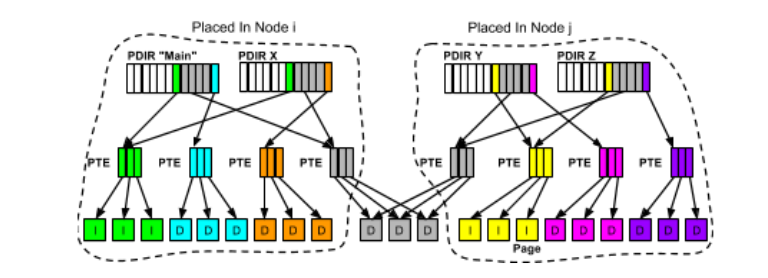
\includegraphics[width=\textwidth]{almos-page-table}
        \caption{Organisation de la table des pages pour quatre threads d'un
          même processus. Deux threads sont placés sur un cluster $i$, et deux
          sur un cluster $j$. Les threads partagent certaines pages de données
          et d'instructions, parfois entre clusters, mais ont également leurs
          pages privées~\citep{almaless2014universite}.}
        \label{fig:almos-page-table}
      \end{figure}

      L'intérêt des processus hybrides est double:

      \begin{itemize}
        \item on évite le goulot d'étranglement sur la table des pages
        \item les espaces virtuels des threads ne sont plus stockés dans le
          processus mais sont indépendants, on a donc économisé de la place dans
          la mémoire virtuelle du processus
      \end{itemize}

      Cette solution permet de minimiser le coût de la cohérence des tables
      entre tous les réplicas et permet également d'alléger les accès
      atomiques. En effet, une application massivement parallèle minimisera les
      dépendances de données entres threads, et donc les pages communes.\\

      Par manque de temps, ce concept n'a pas été implémenté dans le noyau
      ALMOS. Nous allons donc devoir le mettre en place, avec dans un premier
      temps l'objectif d'avoir une table des pages distribuée entre les
      threads.


    \subsection{Les signaux}

      Dans cette partie, nous allons devoir mettre en place des mécanismes pour
      la transmission des signaux lorsque les threads sont distribués sur
      plusieurs noyaux. En effet, la norme POSIX stipule que la portée des
      signaux est un processus dans son ensemble~\citep{man2015signal}.

      Pour cela, il faudra redéfinir la notion de \texttt{pid}. Un \texttt{pid}
      sera découpé en deux parties \benumline \item la partie haute indiquera la
      valeur du cluster sur lequel s'exécute le thread \item la partie basse
      donnera la valeur classique du \texttt{pid} sur ce
      cluster\eenumline. L'application d'un masque sur le champ \texttt{pid}
      permettra alors d'obtenir l'information souhaitée.

      Enfin, après une migration, un processus enverra sa nouvelle adresse au
      noyau d'origine, qui le modifiera dans sa table des processus. Ainsi, le
      noyau d'origine des processus connait en permanence la localisation de ses
      fils sur la machine. Ce mécanisme nous permet de pouvoir transmettre les
      signaux.


  \section{La DQDT}
  \label{sec:dqdt}

    Cette partie du stage est ``optionnelle''. La ré-implémentation de ce
    composant est un besoin réel pour ALMOS, néanmoins cela implique que les
    étapes présentées précédemment soient finalisées.

    La DQDT, pour \textit{Distributed Quaternary Decision Tree}, est le
    composant d'ALMOS assurant une vision cohérente et temps-réel\footnote{C'est
      un abus de langage qui est fait ici. Nous voulons simplement montrer que
      la DQDT permet d'avoir en permanence les taux d'utilisation des 4096
      processeurs de la plateforme.} de l'utilisation des ressources. Dans la
    version de Ghassan~\citet{almaless2014universite}, la DQDT repose sur des
    serveurs répliqués dans tous les clusters. Chaque cluster physique
    représente une feuille de la DQDT. Ces serveurs récupèrent les informations
    sur l'occupation de la machine (c\oe urs et mémoire), et calculent une
    moyenne d'utilisation pour chaque cluster. Cette information est stockée
    dans un n\oe ud de l'arbre. Chaque étage de l'arbre représente un niveau
    d'abstraction. Comme le montre la figure~\ref{fig:dqdt-logical}, le premier
    niveau, en noir, est celui des clusters physiques. Le second niveau, en
    bleu, regroupe 4 clusters. C'est un cluster logique de niveau 1. Le dernier,
    en rouge, regroupe quatre clusters logiques de niveau 1 dans un cluster
    logique de niveau 2. Ces niveaux sont matérialisés par les étages de
    l'arbre, comme le montre la figure~\ref{fig:dqdt-tree}.\\

    \begin{figure}[ht]
      \begin{subfigure}[b]{0.5\textwidth}
        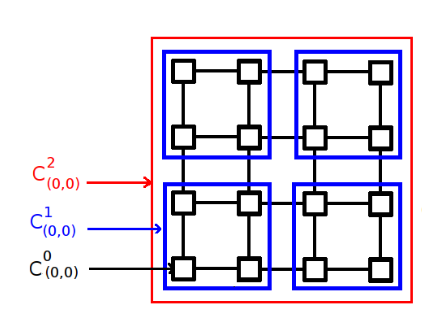
\includegraphics[scale=0.4]{dqdt-logical}
        \caption{Découpage de la plateforme}
        \label{fig:dqdt-logical}
      \end{subfigure}
      \begin{subfigure}[b]{0.4\textwidth}
        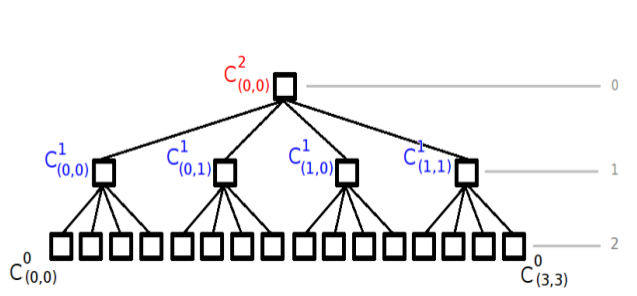
\includegraphics[scale=0.4]{dqdt-tree}
        \caption{Représentation du découpage}
        \label{fig:dqdt-tree}
      \end{subfigure}
      \caption{Construction de la DQDT~\citep{almaless2014universite}.}
    \end{figure}

    La DQDT, comme la plupart des composants noyaux d'ALMOS, repose sur le
    mécanisme de la mémoire virtuelle répartie entre les clusters. Si l'on
    change ALMOS en multi-noyau, les serveurs de la DQDT ne peuvent plus
    communiquer grâce à la mémoire virtuelle. Ils sont obligés d'utiliser le
    passage de messages entre les noyaux.

    Notre but est de changer le schéma de communication de la DQDT. Deux
    techniques peuvent être utilisées:
    \begin{itemize}
      \item avoir une solution portable sur n'importe quelle architecture
        matérielle : nous utilisons le passage de messages
      \item avoir une solution efficace sur l'architecture TSAR : nous profitons
        de mécanismes matériels nous permettant d'accéder directement à la
        mémoire physique des clusters voisins.
    \end{itemize}

    Nous allons dans un premier temps implémenter une version efficace sur TSAR,
    puis selon le temps restant, une solution générique.


    \nomenclature{DQDT}{Distributed Quaternary Decision Tree}
    \nomenclature{RPC}{Remote Procedure Call}
    \nomenclature{UNIX}{Uniplexed Information and Computing Service}
    \nomenclature{PDIR}{Page DIRectory}
    \nomenclature{PTE}{Page Table Entry}


  %% \chapter{Identification des tâches à accomplir}
\label{chap:tasks}


  \section{Processus mono-thread}

    La première étape sera de modifier les \texttt{struct fd\_info\_s} et
    \texttt{struct vfs\_file\_s} gérant la description des fichiers. Nous allons
    mettre en place une des deux tables de hachage présentées au
    chapitre~\ref{chap:sol} pour avoir une nouvelle gestion des
    pointeurs. Précisément, cela nous permettra de retrouver des adresses en
    mémoire après une migration sans avoir besoin de \textit{vrais}
    pointeurs. Nous allons pour cela utiliser les numéros des pages physiques.

    Dans un second temps, nous allons appliquer ce même mécanisme aux régions
    virtuelles partagées. Cette partie est néanmoins optionnelle. Bien
    qu'imposée par la norme POSIX, les régions partagées ne sont pas notre
    priorité. En effet, les processus n'ont par défaut aucune zone partagée. En
    revanche, nous voulons d'abord être capable de gérer les descripteurs de
    fichiers, qui eux sont partagés par défaut : \texttt{stdin, stdout} et
    \texttt{stderr} sont tous les trois des fichiers et sont ouverts par tous
    les processus en permanence.

    Ensuite, nous souhaitons implémenter la fonction de migration qui utilisant
    la DQDT si celle-ci indique qu'une migration doit avoir lieu. Cette fonction
    est spécifique aux processus déjà en cours d'exécution. Nous souhaitons
    également implémenter une fonction permettant de migrer les processus en
    cours de création.
    
    Enfin, nous allons modifier l'appel système \texttt{exec()} pour appeler la
    fonction décrite précédemment.


  \section{Processus multi-thread}

    Notre première étape sera de changer la construction des \texttt{pid} comme
    vu au chapitre~\ref{chap:sol}. Nous devrons ensuite ajouter à la fonction de
    migration un message pour l'envoi du nouveau \texttt{pid} au noyau
    d'origine. Enfin, nous devrons mettre en place un serveur système permettant
    la diffusion des signaux à tous les threads d'un même processus, quelque
    soit leur emplacement sur la machine.

    La seconde étape, la plus délicate, sera l'implémentation du concept des
    processus hybrides. Cette partie s'annonce assez difficile et complexe, en
    particulier la gestion de la table des pages au niveau des threads,
    puisqu'elle touche à la base même d'ALMOS.


  \section{La DQDT}  

    La fonction \texttt{dqdt\_update()} permet de mettre à jour les informations
    sur les taux d'utilisation des processeurs. Cette fonction est appelée
    périodiquement pour assurer une vision correcte de l'utilisation de la
    machine. Nous allons devoir modifier cette fonction selon les techniques
    présentées au chapitre~\ref{chap:sol}, à savoir une méthode générique par
    passage de messages, et une autre plus efficace mais spécifique à notre
    architecture.\\

    Nous pouvons noter que si la DQDT n'est pas opérationnelle, nous pouvons
    quand même valider la migration de processus mono-thread et l'exécution de
    processus multi-thread sur plusieurs clusters. Toutefois, le choix des
    ressources ne sera pas pertinent et les performances seront dégradées, mais
    ce n'est pas important ici. C'est la raison pour laquelle la fonction
    \texttt{dqdt\_update()} est une tâche optionnelle.

  %% \chapter{Définition de la procédure de recette}
\label{chap:tests}

  \todo{chapitre à faire au propre.}\\

  Nous allons à présent donner les différentes procédures de recettes que nous
  allons utiliser pour valider nos solutions.
  
  \section{Migration de processus mono-thread}

    \begin{itemize}
      \item Pour tester les \texttt{fork()} sans \texttt{exec()} : un programme
        C qui \texttt{fork()} à fond et on fait des printfs régulier des
        clusters d'exécution.
      \item Pour tester la migration en cours d'exécution, on devra faire une
        politique ad-hoc dans la DQDT. On fera en sorte qu'au bout d'un temps
        $T$ un processus sera migré sur un autre cluster. Cette modification
        sera faite dans la DQDT. Pour créer ce processus, on peut reprendre le
        programme donné précedemment en ajoutant un appel à \texttt{exec()}
        après le \texttt{fork()}. Chaque processus affiche périodiquement son
        cluster.
    \end{itemize}


  \section{Le multi-threading}

    \begin{itemize}
      \item On reprendre le programme C précédent mais on ajoute en plus la
        création d'un nombre $N$ de thread par processus.
    \end{itemize}


  \section{Évaluation du coût}

    Avec ce qu'on a dit avant, on a de quoi tester la migration mais pas son
    coût en terme de cycles. On va devoir ajouter des compteurs dans les
    programmes pour avoir une idée de la faisabilité de la solution.

  %% \chapter{Échéancier}
\label{chap:sched}

  Nous allons découper notre travail selon l'ordre des tâches présenté au
  chapitre~\ref{chap:tasks}.

  \todo{}

  %% \input{src/results}
  %% \input{src/howto}
  %% \input{src/conclusion}
  %% \input{src/appendix}

  %% For printed version
  \ifx \printed \yes
  \clearpage
  \thispagestyle{empty}
  \cleardoublepage
  \fi

  %% Redefined header for bib
  \fancypagestyle{plain}{
    \fancyhf{}
    \renewcommand{\headrulewidth}{0pt}
    \renewcommand{\footrulewidth}{0pt}
    %% \fancyfoot[RO,LE] {\thepage}
  }
  \pagestyle{plain}
  \bibliographystyle{plainnat}
  \bibliography{src/references}

\end{document}
